\chapter{Creación del sistema}

El sistema que vamos a crear constará de las siguientes partes. Primero sobre las máquinas con SO Windows se instalará una máquina virtual Ubuntu sobre Virtualbox para trabajar en un entorno linux. A día de hoy existen formas de trabajar directamente con Docker en sistemas Windows tanto por CLI (Command Line Interface) como a través de una interfaz gráfica, aunque éstas se basan en emular el kernel de linux. Para este caso se ha optado por trabajar en un entorno linux conocido para hacer más simple el despligue del sistema.

Dentro de dicha máquina Ubuntu se instalará el propio Docker. Mediante Docker crearemos diferentes contenedores. Cada uno de esos contenedores se crearán a partir de una imagen de Ubuntu que vendrá con ROS instalado. Esa imagen sera la que aparece en el Docker Hub como \emph{osrf/ros:indigo-desktop}. Estas máquinas se comunicarán entre ellas mediante una red creada con la herramienta \emph{network} de Docker.

El esquema del sistema vendría a ser el que se muestra en la Figura \ref{fig:esquemaOriginal}.
\begin{figure}[H] % Con el parámetro H la imagens se muestra justo en el sitio en el que se ha definido
	\centering
	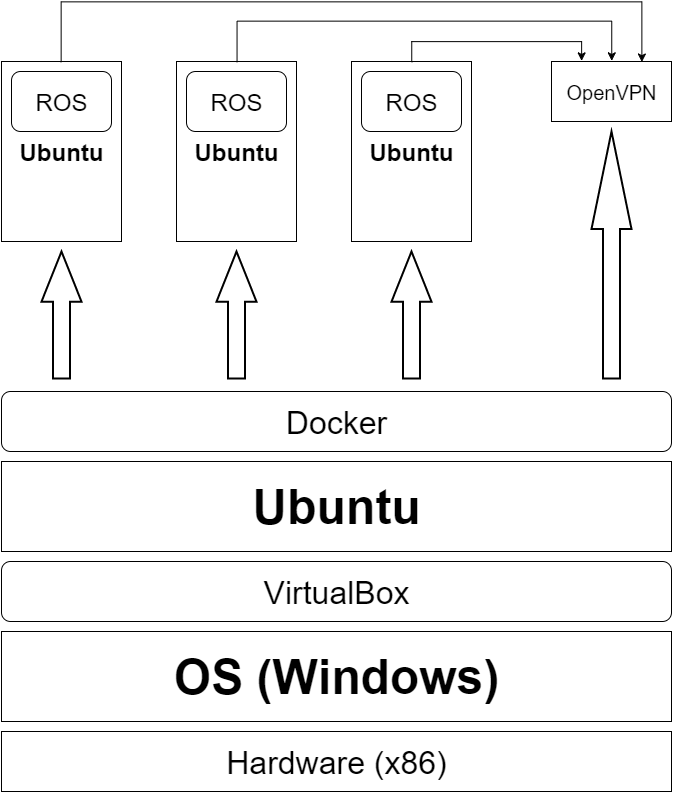
\includegraphics[width=0.8\textwidth]{esquemaOriginal}
	%		\includesvg{figuras/esquemaOriginal}
	\caption{Esquema del sistema en un ordenador x86}
	\label{fig:esquemaOriginal}
\end{figure}

Posteriormente integraremos nuestro sistema en una Raspberry Pi. El esquema del sistema aplicado en una Raspberry Pi se muestra en la Figura \ref{fig:esquemaRPi}.
\begin{figure}[H]
	\centering
	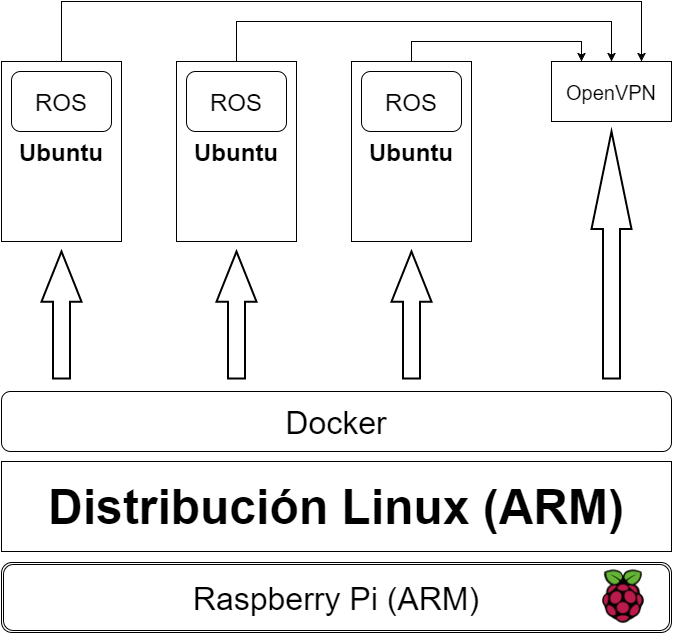
\includegraphics[width=0.8\textwidth]{esquemaRPi}
	%		\includesvg{figuras/esquemaRPi}
	\caption{Esquema del sistema en una Raspberry Pi}
	\label{fig:esquemaRPi}
\end{figure}

	\section{Crear el sistema con Docker}
	Lo primero que haremos será crear una serie de contenedores de docker con ROS dentro.
	
	\begin{enumerate}
		\item Creamos en tres terminales diferentes tres contenedores ROS.
		\begin{lstlisting}[style=consola,numbers=left]
$ docker run --name ros0 -it osrf/ros:indigo-desktop
$ docker run --name ros1 -it osrf/ros:indigo-desktop
$ docker run --name ros2 -it osrf/ros:indigo-desktop
		\end{lstlisting}
		
		\item Desde el host, creamos la red y conectamos los tres contenedores a ella.
		\begin{lstlisting}[style=consola,numbers=left]
$ docker network create red
a9ccfbd91df31be74881c7a7e65fbb0fdd6fec286debec6c72b1f627bb0e2ad0
$ docker network ls
NETWORK ID          NAME                DRIVER
a9ccfbd91df3        red                 bridge              
6fb4fab5cc04        bridge              bridge              
a55fc7d11d74        none                null                
2c96fadb05a4        host                host                
$ docker network connect red ros0
$ docker network connect red ros1
$ docker network connect red ros2
		\end{lstlisting}
		
		\item Probamos el ejemplo anterior con nodos ROS pero esta vez dentro de los contenedores Docker. Simplemente hay que tener en cuenta que hay que configurar la variable \emph{ROS\_MASTER\_URI} para que apunte a \emph{ros0}, que es la dirección del contenedor que ejecutará \emph{roscore}.
		
		\begin{enumerate}
			\item Lanzamos \emph{roscore} en \emph{ros0}.
			\begin{lstlisting}[style=consola]
root@d55b47478e2c:/# roscore
			\end{lstlisting}
			
			\item En \emph{ros1} y \emph{ros2} configuramos la variable que indica donde se está ejecutando \emph{roscore}
			\begin{lstlisting}[style=consola]
$ ROS_MASTER_URI=http://ros0:11311/
			\end{lstlisting}
			
			\item Tanto para \emph{ros1} como para \emph{ros2}, hace falta poner en la variable \emph{ROS\_IP} la IP del conentedor. Esto sirve para que el \emph{roscore} pueda encontrar los nodos. Lo haremos mirando dentro de cada contenedor la IP \textbf{correspondiente a la red creada por nosotros}. En nuestro caso se haría de la siguiente manera.
			\begin{lstlisting}[style=consola]
root@9d1dbcbf599c:~/catkin_ws# export ROS_IP=172.18.0.4
root@ee37147629e4:~/catkin_ws# export ROS_IP=172.18.0.3
			\end{lstlisting}
			
			\item Con todo el ejemplo creado y compilado dentro de \emph{ros1} y \emph{ros2}, lanzamos en \emph{ros1} el listener.
			\begin{lstlisting}[style=consola]
root@9d1dbcbf599c:~/# rosrun prueba listener	
			\end{lstlisting}
			
			\item Y probamos a escribir mediante el talker.
			\begin{lstlisting}[style=consola]
root@9d1dbcbf599c:~/# rostopic pub -1 /chatter std_msgs/String PruebaMensaje
			\end{lstlisting}
			\begin{lstlisting}[style=consola]
root@9d1dbcbf599c:~/# rosrun prueba listener
[ INFO] [1447688515.499505438]: I heard: [PruebaMensaje]
			\end{lstlisting}

		\end{enumerate}
		
	\end{enumerate}
	
	\section{Aplicaciones para el sistema}
		{\color{red} ...en desarrollo}